


\subsection{Output Analysis of $S(d)$}


  \subsubsection{Periodic Boundary Conditions}

      \begin{figure}
         \centering
         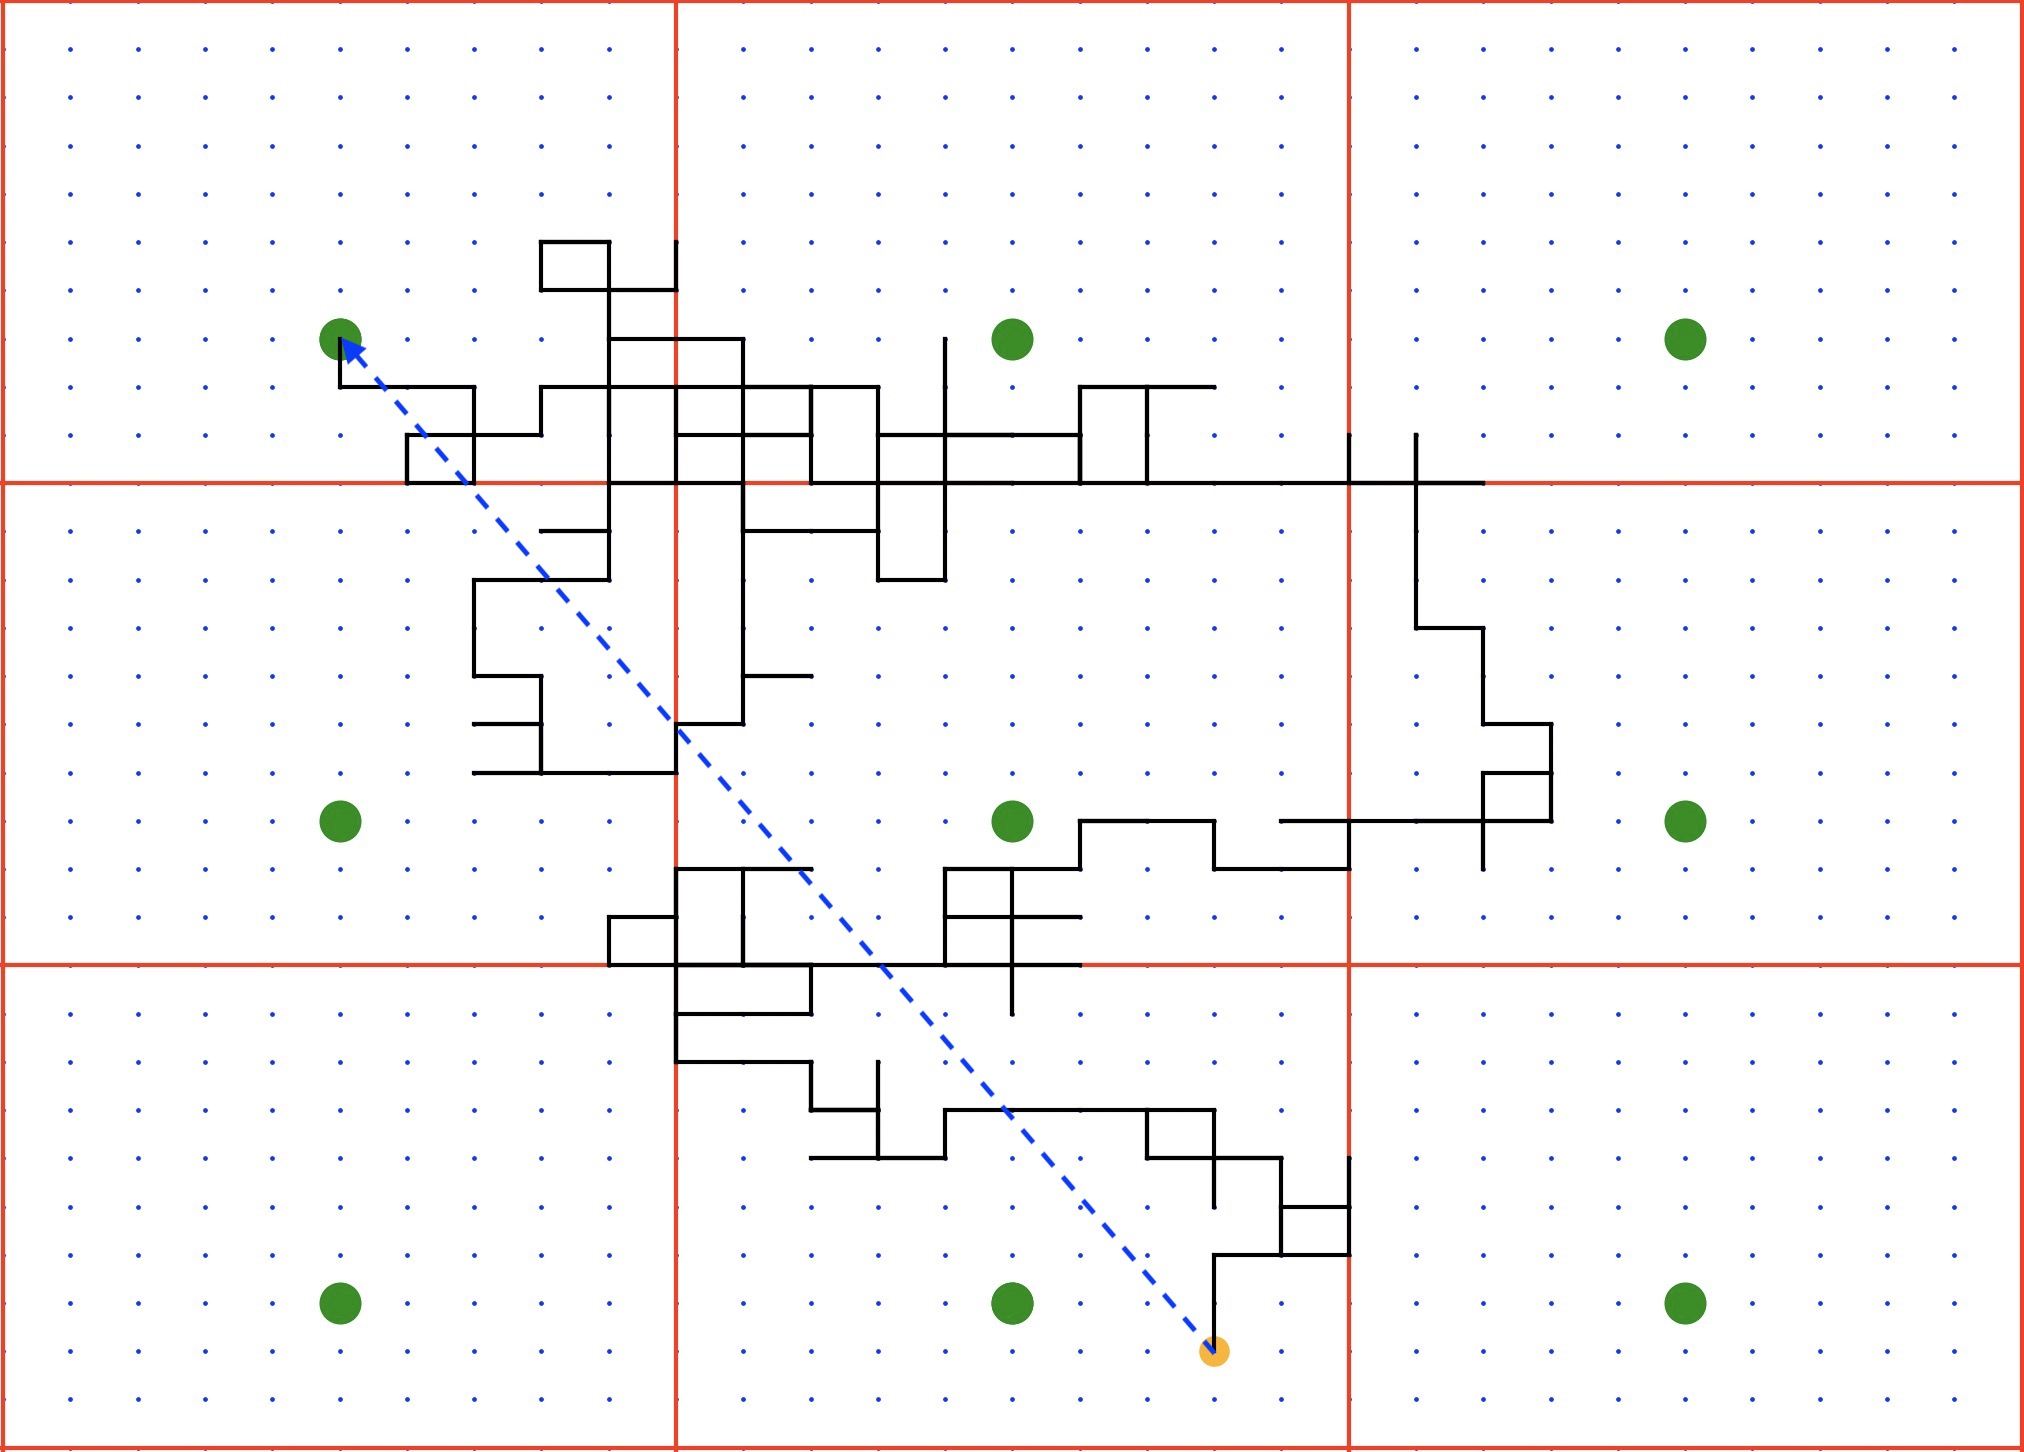
\includegraphics[width=\textwidth]{lrw_perodic_bc.png}
         \caption{This plane is constructed by choosing a primitive
           cell with four red sides and a green point and replicating
           it infinitely to tile the whole $2-$ dimensional
           space. Moreover, there has no overlaps and voids between
           copies of the cell. A particle initially started LRWs from
           the orange site and be absorbed by any of the green points.
           To ensure smoothness and consistency, if the particle
           leaves the cell through one edge, it will appear in the
           adjacent cell with the same velocity. The black line
           segments show the particle's random trajectories, and the
           length of the blue dotted arrow is defined as its
           displacement.}
         \label{fig:pbc_lrws}
      \end{figure}


      In this thesis, periodic boundary conditions (PBCs) are employed
      to minimize the influence of images'
      edges. Fig.~\ref{fig:pbc_lrws} is a simplest example of
      implementing PBCs in the Euclidean plane $E^2$ and tracks the
      trajectory of a particle undergoing LRWs. 




    \subsubsection{Relationship between $n$ and $d$}

     In this section, the displacement of a particle, $d$, is the
     shortest distance from the initial to the stop position in the
     infinite tiling plane. In theory, the mean square displacement
     (MSD) of $N$ Brownian particles at $n-$th step in $2-$dimensional
     space is defined as

     \begin{equation}\label{eq:mds_N}
       MSD = \langle \lvert \bm{r}(n) \lvert^2 \rangle = \frac{1}{N} \sum^{N}_{i=1} (\bm{s}_{i}(n) - \bm{s}_{i}(0))^2 = 4Dn
     \end{equation}
     where the subscript, $i$, refers to each particle for which the
     MSD is calculated. $\bm{s}_{i}(n)$ and $\bm{s}_{i}(0)$ are the
     $i-$th particle positions at $n-$th step and at the initial time,
     respectively. $D$ is diffusion coefficient which is related to
     the variance of the independent displacements of the
     particle. In the simulation, $D$ equals $1$.


     Eq.~\ref{eq:mds_N} indicates a linear relationship between the
     mean square displacement of the particle and the number of
     steps. It is a feature of the normal diffusive
     behavior. Fig.~\ref{fig:G_1_L_3_msd_n} shows how the difference
     between MSD of the particle and $4n$ varying over $\log_{10}n$ in
     LRWs in $G_1L_3$. Moreover, the points are divided into several
     subgroups based on various intervals of steps, and their colours
     are as identical as the segments in
     Fig.~\ref{fig:steps_seg_curve_G_1_L_3}. When $n \leq 4064.0$, the
     variation is not equal to $0$ with larger fluctuation, which
     implies that blue, yellow, and pink particles undergo anomalous
     diffusion process. In other words,

     \begin{equation}\label{eq:anomalous_diffusion}
       \langle \lvert \bm{r}(n) \lvert^2 \rangle \propto n^{\gamma}
     \end{equation}
     where $\gamma \ne 1$. In Fig.~\ref{fig:steps_seg_curve_G_1_L_3},
     positive variation implies $\gamma < 1$ called subdiffusion
     process, while negative value denotes $\gamma > 1$ named
     superdiffusion.

     
      
      \begin{figure}
         \centering
         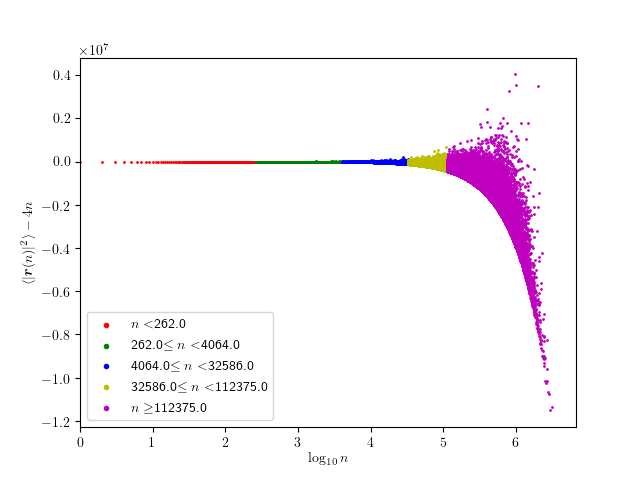
\includegraphics[width=\textwidth]{G_1_L_3_msd_n.png}
         \caption{}
         \label{fig:G_1_L_3_msd_n}
      \end{figure}

      \begin{figure}
         \centering
         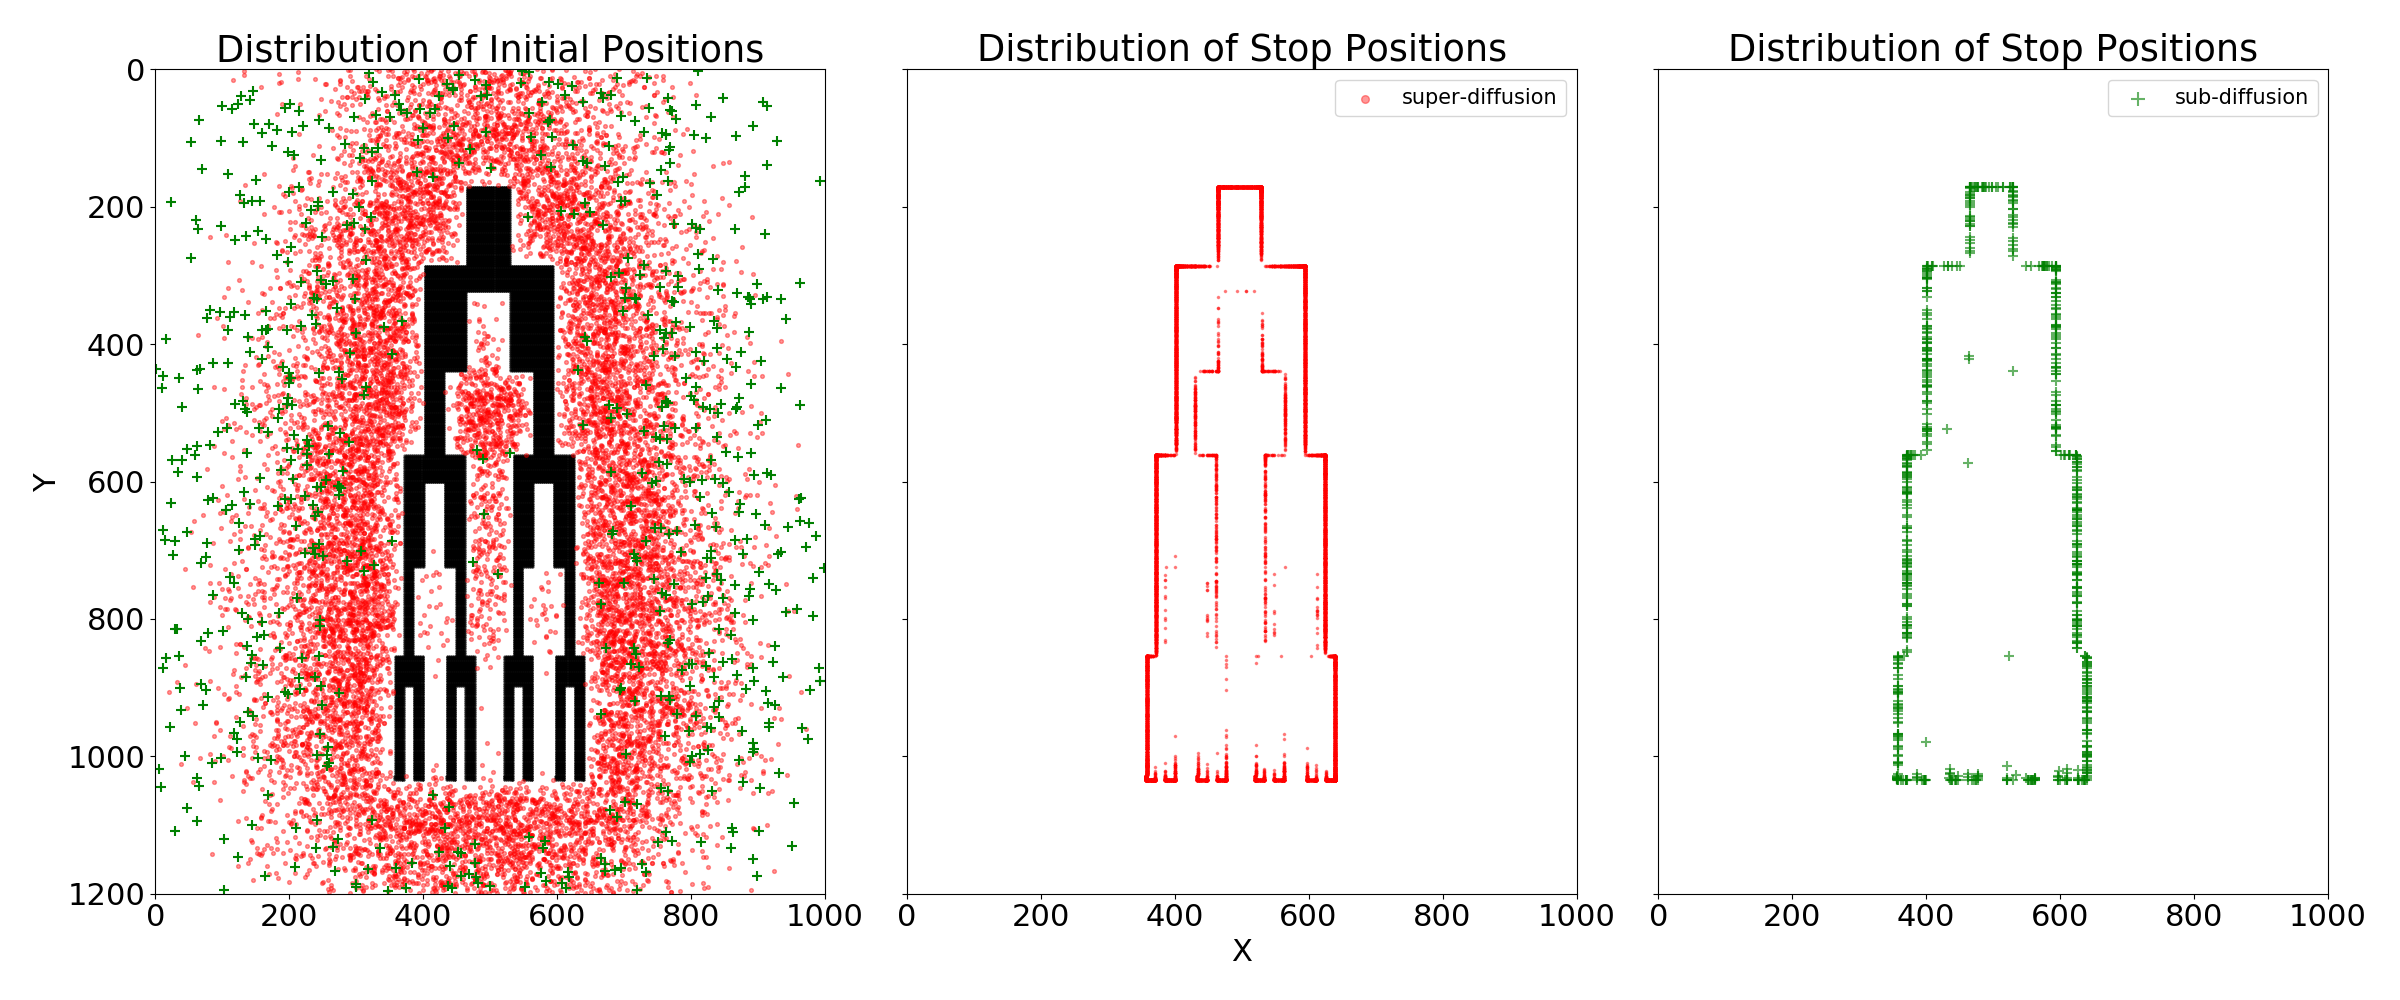
\includegraphics[width=\textwidth]{G_1_L_3_steps_blue_initial_stop_pos_var.png}
         \caption{}
         \label{fig:G_1_L_3_var_initial_stop_pos}
      \end{figure}

      
      

      \begin{figure}
        \centering
        
        \begin{subfigure}[b]{0.45\textwidth}
          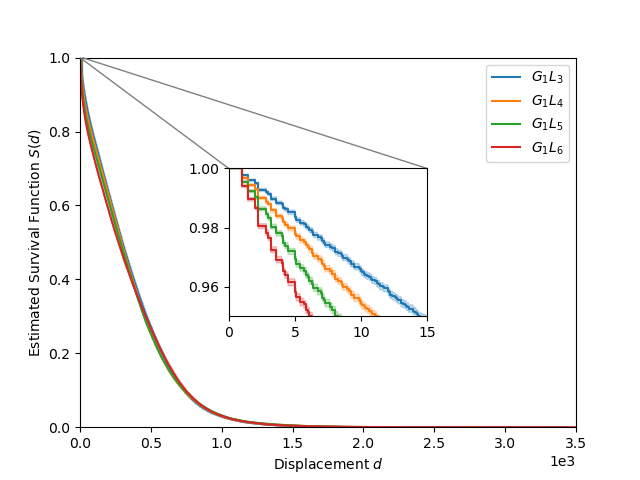
\includegraphics[width=\textwidth]{G_1_unwrap_disp_sf.png}
          \caption{}
          \label{fig:sf_g1_branch_disp}
        \end{subfigure}
        \hfill
        \begin{subfigure}[b]{0.45\textwidth}
          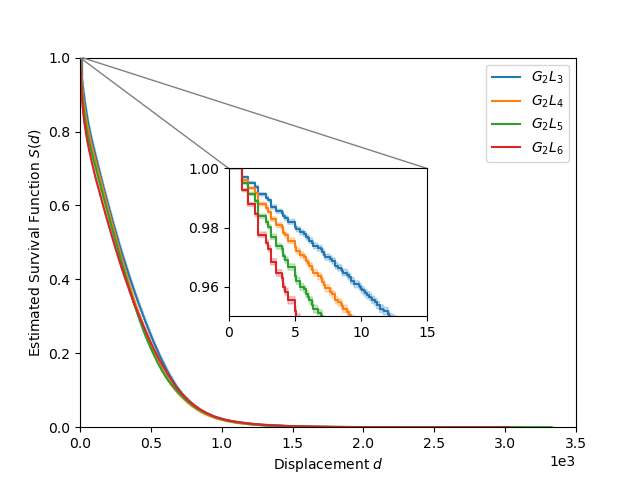
\includegraphics[width=\textwidth]{G_2_unwrap_disp_sf.png}
          \caption{}
          \label{fig:sf_g2_branch_disp}
        \end{subfigure}

        \caption{}
        \label{fig:sf_branch_disp}

      \end{figure}




      \begin{figure}
         \centering
         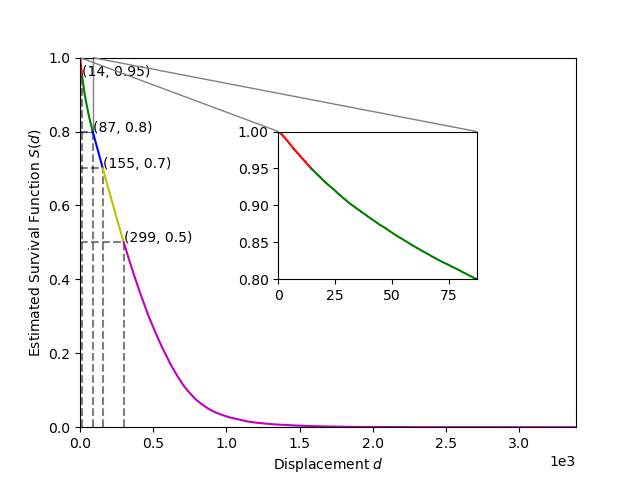
\includegraphics[width=\textwidth]{unwrap_disp_seg_curve_G_1_L_3.png}
         \caption{}
         \label{fig:disp_seg_curve_G_1_L_3}
      \end{figure}

      
       \begin{figure}
         \centering
         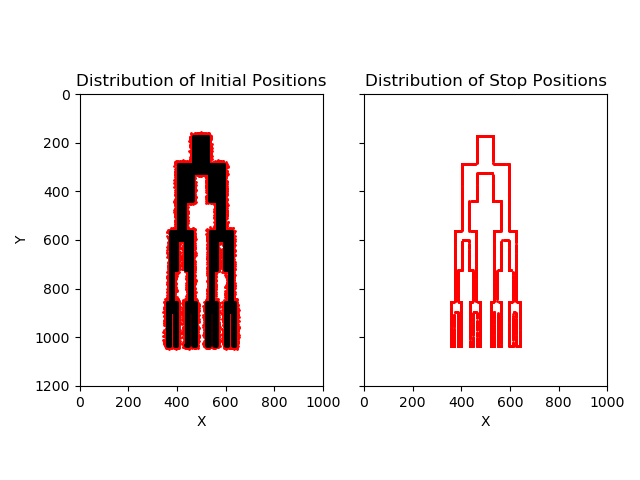
\includegraphics[width=\textwidth]{G_1_L_3_unwrap_disp_red_initial_pos_distribution.png}
         \caption{}
         \label{fig:G_1_L_3_disp_red_initial_pos_distribution}
       \end{figure}


       \begin{figure}
         \centering
         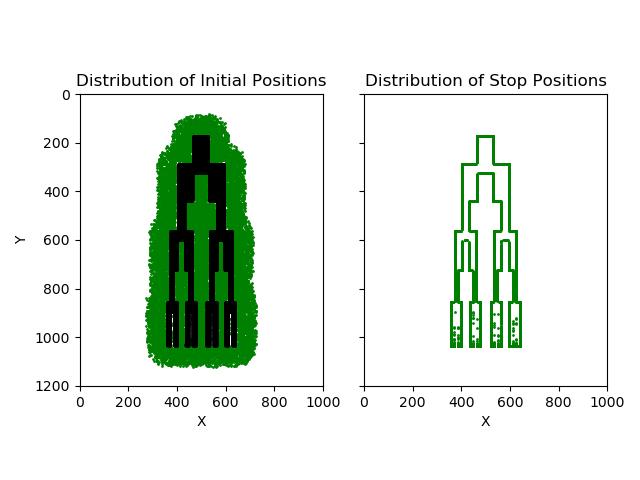
\includegraphics[width=\textwidth]{G_1_L_3_unwrap_disp_green_initial_pos_distribution.png}
         \caption{}
         \label{fig:G_1_L_3_disp_green_initial_pos_distribution}
       \end{figure}


        \begin{figure}
         \centering
         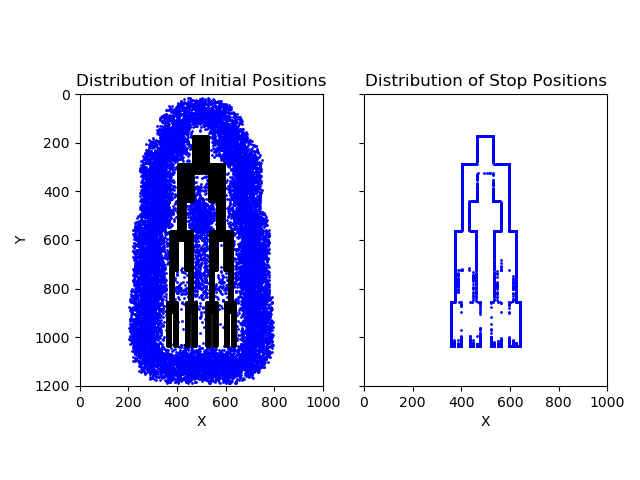
\includegraphics[width=\textwidth]{G_1_L_3_unwrap_disp_blue_initial_pos_distribution.png}
         \caption{}
         \label{fig:G_1_L_3_disp_blue_initial_pos_distribution}
        \end{figure}


        \begin{figure}
         \centering
         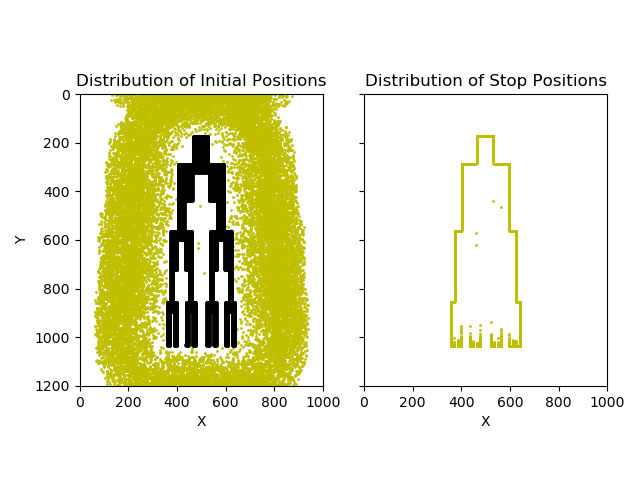
\includegraphics[width=\textwidth]{G_1_L_3_unwrap_disp_y_initial_pos_distribution.png}
         \caption{}
         \label{fig:G_1_L_3_disp_yellow_initial_pos_distribution}
        \end{figure}



        \begin{figure}
         \centering
         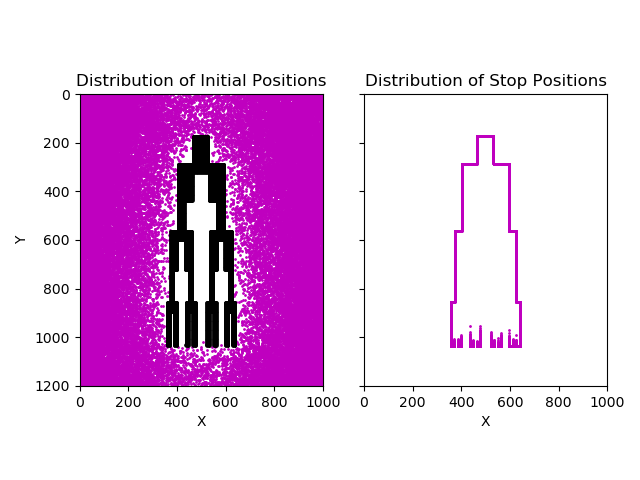
\includegraphics[width=\textwidth]{G_1_L_3_unwrap_disp_m_initial_pos_distribution.png}
         \caption{}
         \label{fig:G_1_L_3_disp_pink_initial_pos_distribution}
        \end{figure}


        

        \begin{figure}
        \centering
        \begin{subfigure}[b]{0.45\textwidth}
          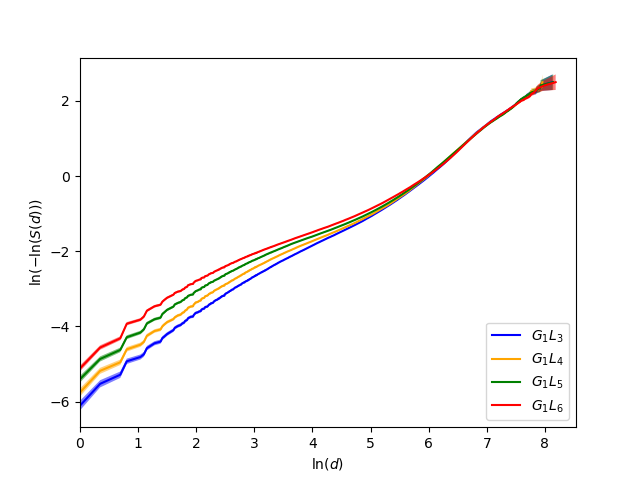
\includegraphics[width=\textwidth]{G_1_unwrap_disp_check_ph.png}
          \caption{}
          \label{fig:g1_disp_check_ph}
        \end{subfigure}
        \hfill
        \begin{subfigure}[b]{0.45\textwidth}
          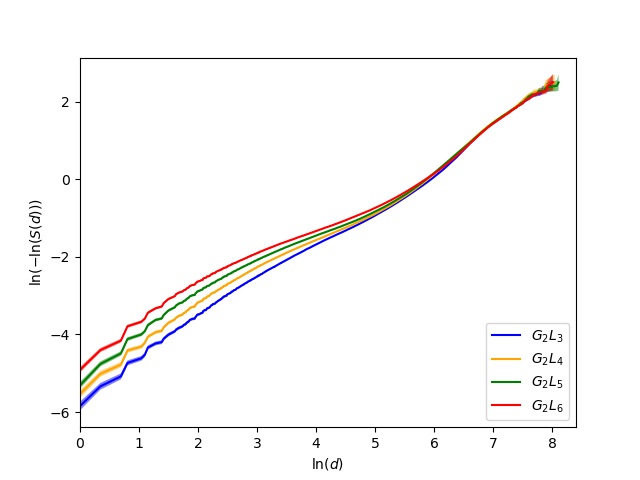
\includegraphics[width=\textwidth]{G_2_unwrap_disp_check_ph.png}
          \caption{}
          \label{fig:g1_disp_check_ph}
        \end{subfigure}
        \caption{}
        \label{fig:branch_disp_check_ph}
      \end{figure}

        
      

      \begin{table}
        \centering
        \begin{tabular}{llrrrr}
          \toprule
                       &             &         &  p &    &     \\
          \cmidrule{3-6}
                       &             & Logrank & TW & GB & FH  \\
          \midrule
          $G_1$ $L_3$  & $G_1$ $L_4$  &  0.0 &  0.0 &  0.0 &  0.0     \\
                       & $G_1$ $L_5$  & 0.0 & 0.0 & 0.0 & 0.0    \\
                       & $G_1$ $L_6$  & 0.0 & 0.0 & 0.0 & 0.0      \\
          $G_1$ $L_4$  & $G_1$ $L_5$  & 0.0072 & 0.0 & 0.0 & 0.0      \\
                       & $G_1$ $L_6$  & 0.0003 & 0.0 & 0.0 & 0.0       \\
          $G_1$ $L_5$   & $G_1$ $L_6$ & 0.2883 &  0.0 & 0.0 & 0.0      \\
          \bottomrule
        \end{tabular}
        \label{tab:g1_ingroup_tests_disp}
        \caption{}
      \end{table}


      \begin{table}
        \centering
        \begin{tabular}{llrrrr}
          \toprule
                       &             &         &  p &    &     \\
          \cmidrule{3-6}
                       &             & Logrank & TW & GB & FH  \\
          \midrule
          $G_2$ $L_3$  & $G_2$ $L_4$  &  0.0 &  0.0 &  0.0 &  0.0     \\
                       & $G_2$ $L_5$  & 0.0 & 0.0 & 0.0 & 0.0    \\
                       & $G_2$ $L_6$  & 0.0 & 0.0 & 0.0 & 0.0      \\
          $G_2$ $L_4$  & $G_2$ $L_5$  & 0.0001 & 0.0 & 0.0 & 0.0      \\
                       & $G_2$ $L_6$  & 0.0015 & 0.0 & 0.0 & 0.0       \\
          $G_2$ $L_5$   & $G_2$ $L_6$ & 0.7019 &  0.0 & 0.0 & 0.0      \\
          \bottomrule
        \end{tabular}
        \label{tab:g2_ingroup_tests_disp}
        \caption{}
      \end{table}



      

      \begin{figure}
        \centering
        \begin{subfigure}[b]{0.45\textwidth}
          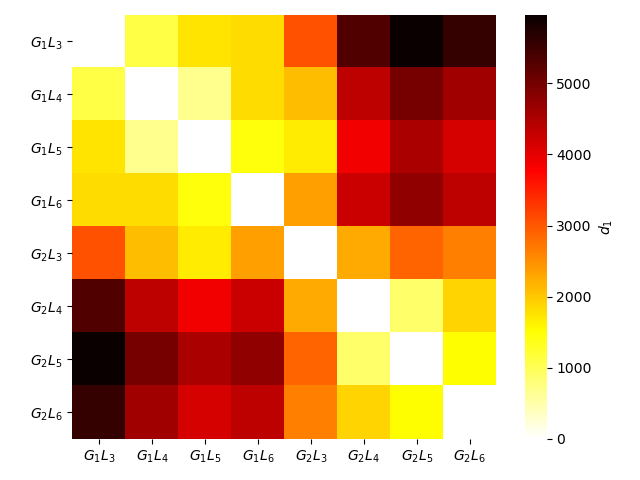
\includegraphics[width=\textwidth]{heatmap_ai_disp_l1.png}
          \caption{}
          \label{fig:heatmap_ai_disp_l1}
        \end{subfigure}
        \begin{subfigure}[b]{0.45\textwidth}
          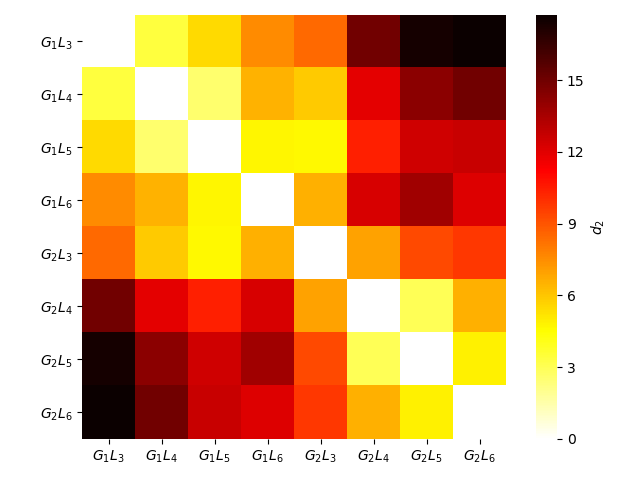
\includegraphics[width=\textwidth]{heatmap_ai_disp_l2.png}
          \caption{}
          \label{fig:heatmap_ai_disp_l2}
        \end{subfigure}
        \caption{}
        \label{fig:heatmap_ai_disp}
      \end{figure}
      
